% ============================================================
% Appendix C: Test Log Format and Measurement Capture
% ============================================================
\chapter{Test Log Format and Measurement Capture}
\label{app:test_logs}

This appendix illustrates the format of the system-level test log and contains the archived oscilloscope capture of the watchdog test.

% ------------------------------------------------------------
\section{System-Level Test Log Format}
\label{sec:app_system_log_excerpts}

The following excerpt illustrates the format of the log written by the fixture application~\cite{dolata2023}; it is a reconstruction, the fields in brackets are placeholders, and no raw log of these tests was archived. The long description line is wrapped for printing. In the header, \texttt{Tester} holds the person carrying out the tests and \texttt{Cart ID} the identifier of the board under test; the requirements of the fixture ask the log to record both~\cite[Sec.~3.1.5]{dolata2023}.

\subsection*{Example: Log Format for a Fault Memory Cycle Test (\texttt{Geber 3})}

{\footnotesize
\begin{verbatim}
--------------------------------------------------
Logging test results using version 1.0

Tester: [name]
Cart ID: [board identifier]

Date: [YYYY-MM-DD]
Time: [hh:mm:ss]
--------------------------------------------------

--------------------------------------------------
Test: Geber 3 - I
Description: Test für den Geber. Bitte 3 Sekunden warten,
    bis der Fehler angezeigt wird. Danach STW gedrückt halten
    und Fehlersequenz überprüfen.
expected_err_code: 31
expected_err_seq: 03 31 09
Comment: [observation]
Result: [PASS/FAIL]
--------------------------------------------------
... [Additional test steps for other fault conditions] ...
--------------------------------------------------
\end{verbatim}
}

\clearpage

% ------------------------------------------------------------
\section{Measurement Capture}
\label{sec:app_verification_captures}

No measurement of the watchdog reaction or of the frequency sweep on the rebuilt unit is documented (\Cref{subsec:fpga_interface_results}). The capture below was taken by Leyer on the inherited Rev~0.0 prototype in 2023~\cite{leyer2023}, like the emulation's sweep in~\Cref{fig:sweep_comparison}. It documents the measurement method of Layer~1 (\Cref{sec:fpga_interface_testing}) on the prototype. It is not a reference from the original board, whose watchdog could not be observed, and the reset interval it shows is the prototype's, which Leyer doubted (\Cref{subsec:fpga_interface_results}).

\begin{figure}[htbp]
	\centering
	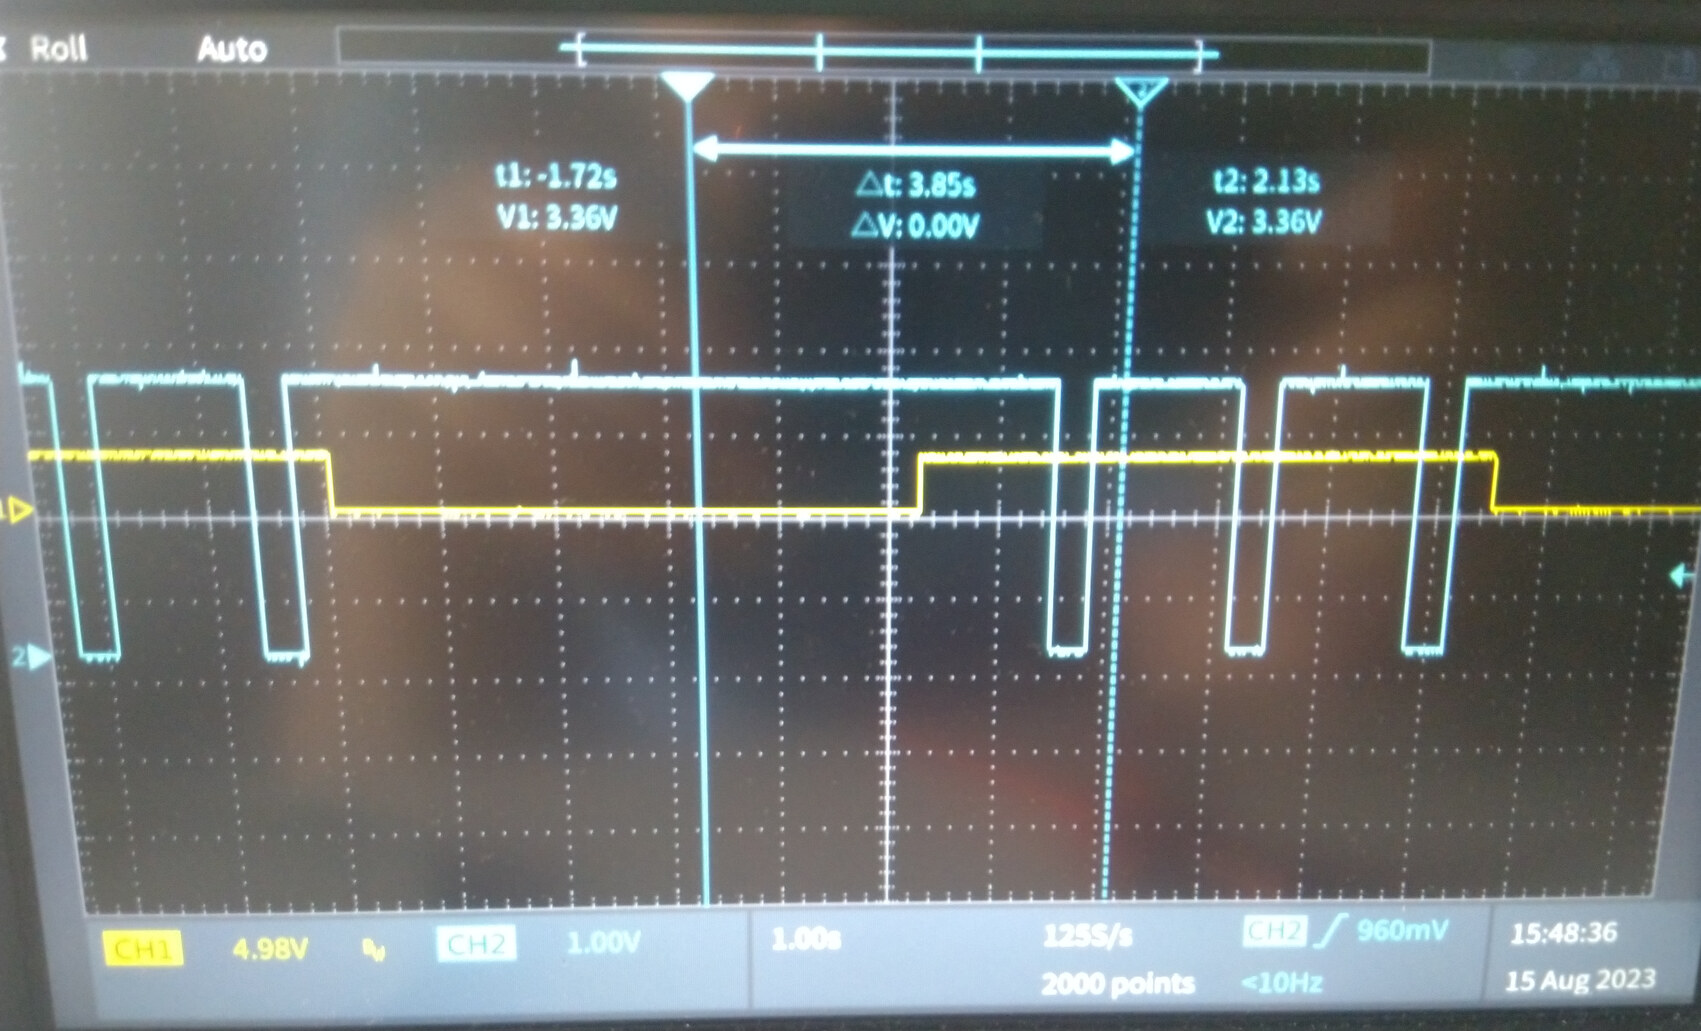
\includegraphics[width=0.9\textwidth]{watchdog_capture.jpg}
	\caption[Watchdog Reset Test on the Rev 0.0 Prototype]{Watchdog reset test on the inherited Rev~0.0 prototype (oscilloscope date stamp 15~August~2023). A test design in the \gls{fpga} toggles the watchdog service line about every \SI{20}{\milli\second} for about five seconds (256 times) and then withholds service, so that the watchdog pulls the controller reset low; Leyer expected a reset every \SI{1.2}{\second} and doubted the value~\cite[Sec.~4.6]{leyer2023}. Read from the photograph, the first reset follows about \SI{1.2}{\second} after the service stops, and resets of about \SI{0.3}{\second} recur about \SI{1.6}{\second} apart (\Cref{subsec:fpga_interface_results}). Yellow: service line, inverted before the watchdog (the individual pulses are not resolved); blue: controller reset line. The cursor readout ($\Delta t = \SI{3.85}{\second}$, \SI{3.36}{\volt}) measures no watchdog parameter; the voltage is the cursor level. Reproduced from~\cite[Fig.~9]{leyer2023}, cropped to the screen from the archived photograph.}
	\label{fig:watchdog_reaction}
\end{figure}
